\documentclass{beamer}
\usepackage[utf8]{inputenc}
\usepackage{graphicx}
\author[Sowmya Vajjala]{Instructor: Sowmya Vajjala}


\title[LING 120]{LING 120, Fall 2017 \\ Language and Computers}

\date{18 September 2017}

\institute{Iowa State University, USA}

%%%%%%%%%%%%%%%%%%%%%%%%%%%

\begin{document}

\begin{frame}\titlepage
\end{frame}

\begin{frame}
\frametitle{Class outline}%5minutes
\begin{enumerate}
\item Recap of Week 4
\item Introduction to Search
\item Language and Search
\end{enumerate}
\end{frame}

%Last week's question
\begin{frame}
\frametitle{Last class' Exercise}
Assume you are given the task of designing a software that can automatically score short answers from students about whatever they read (science, maths, any subject). 
How will you go about this? What kind of tasks should that system do? What are the features we should look at to evaluate student answers? \\
a) if we have a target answer \\
b) if we do not have a target answer
\\ \medskip (write your answers on a sheet of paper and return to me. You can also post on Canvas in the discussion forum for today's date)
\end{frame}

\begin{frame}
\frametitle{Your Responses: When we have a target answer}%5minutes
\begin{enumerate}
\item Keyword/phrase/n-gram match with target answers (similar to a plagiarism detector!) \pause
\item There should be large database of semantic relationships between words - so that we can capture words that are not exactly as target answer but similar.  \pause
\item Paraphrasing of target answers should be identified \pause 
\end{enumerate}
\end{frame}

\begin{frame}
\frametitle{Your Responses: When we do not have a target answer}%5minutes
\begin{enumerate}
\item Look for words around the words in the question, and compare the words in answers with them. \pause
\item Take a probability based approach. If there is no target answer, and there are lot of student answers, we can assume that the frequent answer is the right answer, and go from there. \pause
\item Computer should read the text the student read and figure out answer to the question, and then compare student answer with it. 
\end{enumerate}
\end{frame}

\begin{frame}
\frametitle{So how do people solve this?}%5minutes
\begin{enumerate}
\item Scoring of maths and science responses, and general content: m-rater, science rater and c-rater by ETS
\item Kaggle-Short Answer Assessment Prize : \url{https://www.kaggle.com/c/asap-sas}
% (ETS-Maths) %https://www.ets.org/Media/Research/pdf/RM-11-12.pdf 
\item Cognii.com demo \\ \url{http://cognii.com/demo} \pause
\item Going from that question to our next topic: 
\begin{itemize}
\item Searching for right answers: \url{https://www.youtube.com/watch?v=HXIfwL2-4Ek}
\item Asking the right questions: \url{https://www.youtube.com/watch?v=UIzcIC5RQN8}
\end{itemize}
\end{enumerate}
\end{frame} %15min until here.

\begin{frame}
\frametitle{Topic 4: Search}%5minutes
\begin{enumerate}
\item Introduction to Search (today)
\item Searching through structured vs unstructured data (today)
\item Searching the Web (rest of this week) %Regex Next week 
\item Searching with regular expressions (next week)
\item Searching through large text corpora (next week)
\end{enumerate}
\end{frame}

\begin{frame}
\frametitle{Warmup questions}%5minutes
\begin{enumerate}
\item How many of you use a search engine (google, bing etc)? \pause
\item How do you use it? (browser/mobile, voice/text etc) \pause
\item Other than a search engine, where did you have to "search" for information? \pause
\item What kinds of information, in your opinion is easy to search? \pause
\item How do you search for images or music files? \pause
\end{enumerate}
\end{frame}

\begin{frame}
\frametitle{Searching is questioning/querying}%5minutes
\begin{enumerate}
\item We keep querying, and updating our queries, until we find the results of our search.
\item Note: We also have other possible ways to obtain this information - if you already know where to look for. 
\item Search can be related to any form of data (text, speech, image)
\item The data we are searching for can be of different types: structured, unstructured, semi-structured data.
\end{enumerate}
\end{frame}

\begin{frame}
\frametitle{Different types of data}%5minutes
\begin{enumerate}
\item Structured - Very organized (e.g., a library database - every book has a title, an author, a publisher, other attributes such as number of pages etc.)
\item Unstructured - free-flowing text from which we should extract what we want (e.g., your typical google search)
\item Semi-structured - where the data is generally unstructured, but there are certain patterns we see, which makes it easy to extract content (e.g., if we want to extract all email addresses from a text).
\end{enumerate}
\end{frame}

\begin{frame}
\frametitle{Searching through Structured Data}%5minutes
\begin{enumerate}
\item It is actually quite easy to search through structured data. (Why?) \pause
\item So, what is the problem? Why can't we just work with structured data? \pause
\item Have you used lib.iastate.edu to search for books or other stuff before? Is there some structure in the search or is it totally unstructured? \pause
\item On lib.iastate.edu, if I search for "(energy OR effort) AND student success", what does that mean? Is this what we could call structured data? or is it just structured search?
\end{enumerate}
\end{frame}

\begin{frame}
\frametitle{Searching through UnStructured Data}%5minutes
\begin{enumerate}
\item What is similar to structured data: Here too, you have to search by some keywords or phrases. 
\item Problems: explicit categorization does not exist for text. So, it is not easy to find what you want. \pause
\item It is also very difficult if you have billions of files all over the web, in a WWW search. Should we go through all the files?
\item How do the search engines show search results almost instantly, then?
\end{enumerate}
\end{frame}

\begin{frame}
\frametitle{Evaluating Search Results}%5minutes
\begin{enumerate}
\item We know how to evaluate search results based on our information need. How do we decide whether a search system is generally good? \pause
\item Relevance: Whether the result a search showed us is actually relevant for the user's need. \pause
\item Precision: Of all results returned by the search, how many are actually relevant?
\item Recall: Of all the results that are relevant, how many did the search engine manage to retrieve as relevant? 
\item The goal of a good search engine is to provide 100\% precision and 100\% recall. 
\end{enumerate}
\end{frame}

\begin{frame}
\frametitle{Precision and Recall: Competing Priorities}%5minutes
\begin{enumerate}
\item How do we achieve 100\% recall? \pause
\\ $\Rightarrow$ Just show up everything in the world - that will automatically achieve 100\% recall (How??) \pause
\item How do we achieve 100\% precision? \pause
\\ $\Rightarrow$ return that small set of webpages which you are absolutely sure of. (Great, what is the problem then?) \pause
\item Often, the goal is to reach a balance between precision and recall. 
\end{enumerate}
\end{frame}

%One-Two slides on features of a search Engine
%Examples of ambiguous words and grouping of search results etc.
%Examples of typos
%

\begin{frame} %10-15 min
\frametitle{Attendance Exercise: A question about "searching"}
Work in groups of 2--3 people, think about a solution for this problem, and return your answers to me giving the names of your team members. You can also submit online on Canvas. 
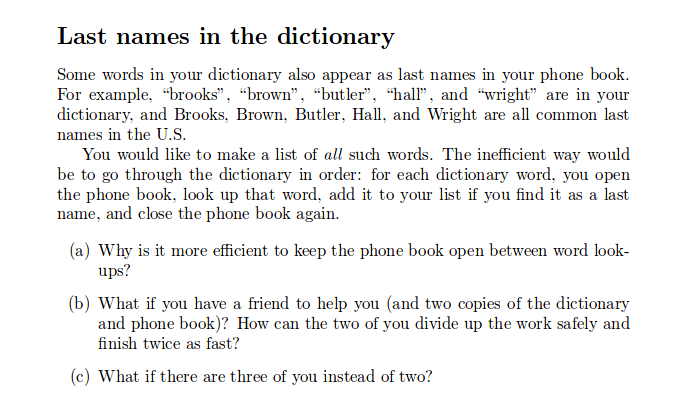
\includegraphics[width=0.9\textwidth]{18Sep-120Exercise.png}
\tiny source: \url{http://nacloweb.org/resources/problems/sample/Phonebook.pdf}
\end{frame}
%solution: http://nacloweb.org/resources/problems/sample/Phonebook-solution.pdf

\end{document}

%Friday problem: Pooh's encyclopaedia problem - http://www.nacloweb.org/resources/problems/2007/prob07.pdf
